\label{membrane:chapter}
In this section, we compare the conformation of FAK bound to a \pip{}-containing membrane (FAK-MEM) to the observations of FAK-SOL in order to get an insight into conformational changes due to \pip{}. To this end, FAK structures of setup 4 were used with the condition that the FAK molecules have no neighbours.\\
\\
The distribution of $d_\text{F2-C}$ shown in \autoref{mem:comdist} lacks the peak observed for FAK-SOL at $3.8\,\si{\nano\metre}$ which has been associated with spot 1 (see \autoref{free:pic_ca_and_com}). Moreover, the distribution of $d_\text{F1-N}$ shows a distinct peak at values associated to spot 2 observed in FAK-SOL ($4.0\,\si{\nano\metre}$). This implies that the tilting of the kinase domain is suppressed in presence of the membrane, which is reasonable since both, FERM domain and kinase, have a docking site for \pip{}. However, there is a significant increase in the contact area CA of ca. $10\%$ to $30.8\,\si{\nano\metre}^2$ (see \autoref{mem:contactarea}), which suggest a closure of the two domains.\\
%
%
%
\begin{figure}[hb]
	\subcaptionbox{\label{mem:comdist}}[0.49\textwidth]{
		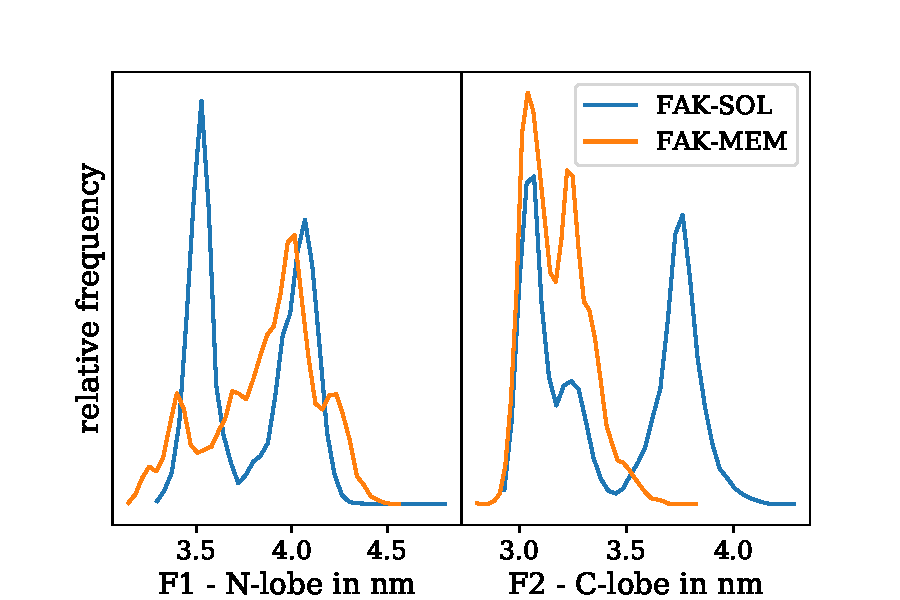
\includegraphics[height=5cm]{figures/results/comp_free_mem_comdist}
	}\hfill%
	\subcaptionbox{\label{mem:contactarea}}[0.49\textwidth]{
		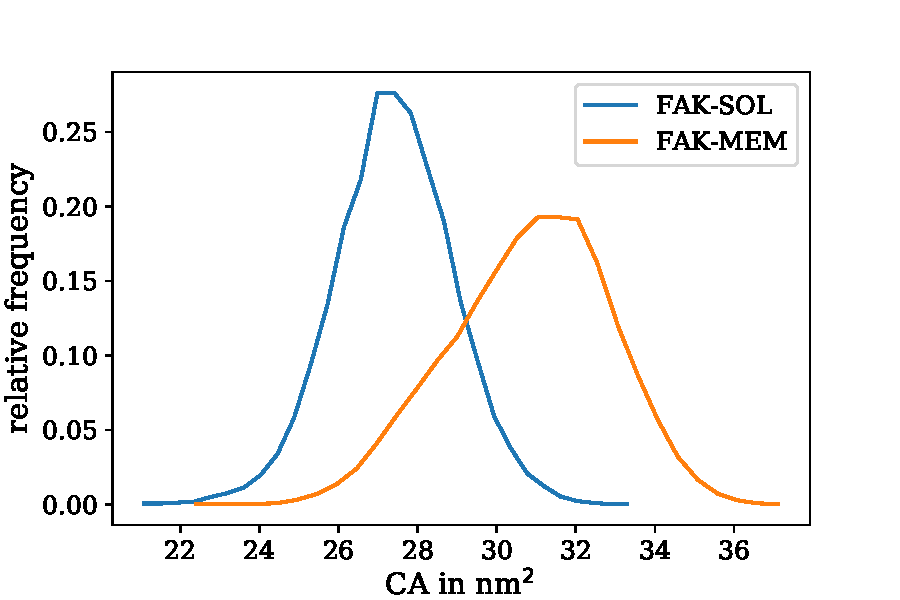
\includegraphics[height=5cm]{figures/results/ca_sol_mem}
	}%
	\nicecaption{Domain distances and contact area of FAK-MEM}{(\subref{mem:comdist}): distribution of $d_\text{F1-N}$ and $d_\text{F2-C}$ in comparison to FAK-SOL. The preferred state corresponds to spot 2 observed in FAK-SOL. (\subref{mem:contactarea}): CA in comparison to FAK-SOL. The mean value is increased by ca. $10\%$.}
\end{figure}
%
%
%
\\
The difference contact map in \autoref{mem:contact} shows the difference of inter-residue distances in comparison to FAK-SOL. At the interface of F2 and the C-lobe (area 1), the residue pairs get closer. In area 2, both increases and decreases in distances can be found. Regarding the 3D structure (\autoref{mem:3d}), one can see that although the upper part of the interface (contacts between \acid{P}{49} to \acid{S}{54} and the kinase, yellow) gets closer, the region below (contacts between \acid{E}{44} to \acid{E}{48} and the kinase, magenta) gets farther away. This induces a spreading of the interface at the activation loop including the activity-regulating residues \acid{Y}{576} and \acid{Y}{577}.\\
Also in the linker region, conformational changes can be observed. Area 3 indicates that the \acid{Y}{397}-containing ball structure observed in FAK-SOL disappears. As shown in \autoref{mem:3d}, the linker is pulled back to the FERM domain, which results in an exposed position of the autophosphorylation site \acid{Y}{397}.\\
\\
As suggested by findings of \textcite{pap001} and \textcite{pap003}, the FERM domain does not dissociate from the kinase because of binding to \pip{}. However, this binding leads to conformational changes resulting in a partial opening of the FERM-kinase interface at the activation loop and the exposure of the autophosphorylation site \acid{Y}{397}.
%
%
%
\begin{figure}[th]
	\centering
	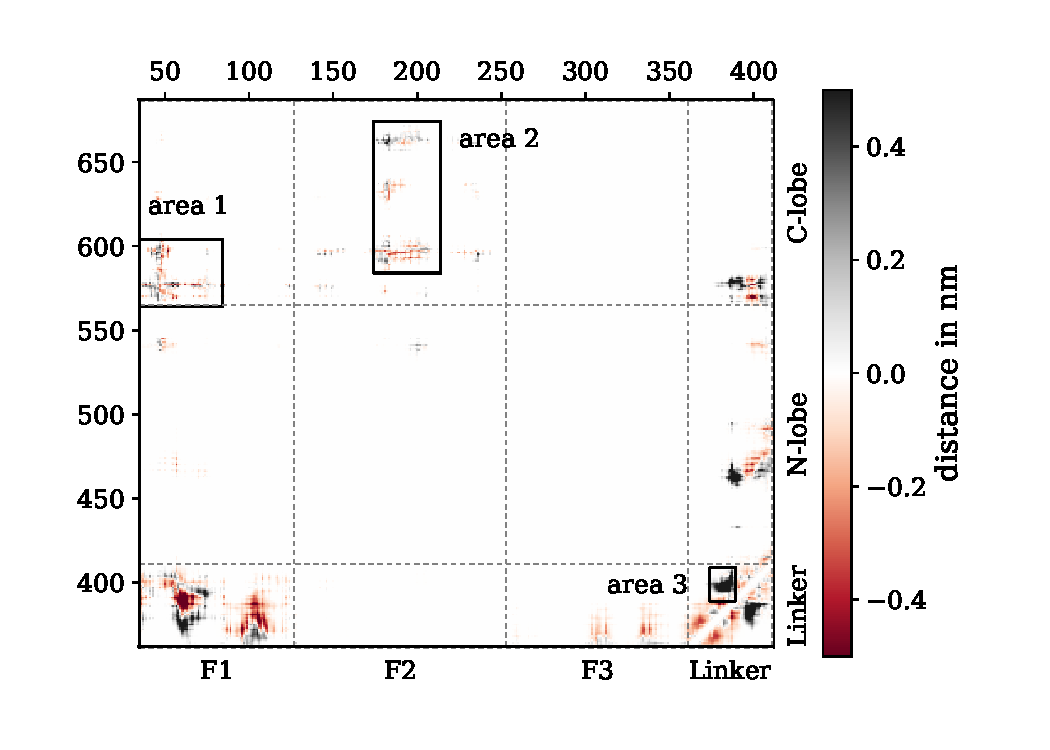
\includegraphics[width=.8\textwidth]{figures/results/contactmap_diff_to_free}
	\nicecaption{Contact map of FAK-MEM}{The contact map shows the difference FAK-MEM - FAK-SOL of the inter-residue distances for the FERM-kinase interface. Conformational changes (area 1 and 2) as well as the exposure of \acid{Y}{397} (area 3) can be seen. The underlying dataset for FAK-MEM is the same as for the correlation contact map in \autoref{force:contactmap}.}
	\label{mem:contact}
\end{figure}
%
%
%
%
%
%
\begin{figure}[hb]
	\centering
	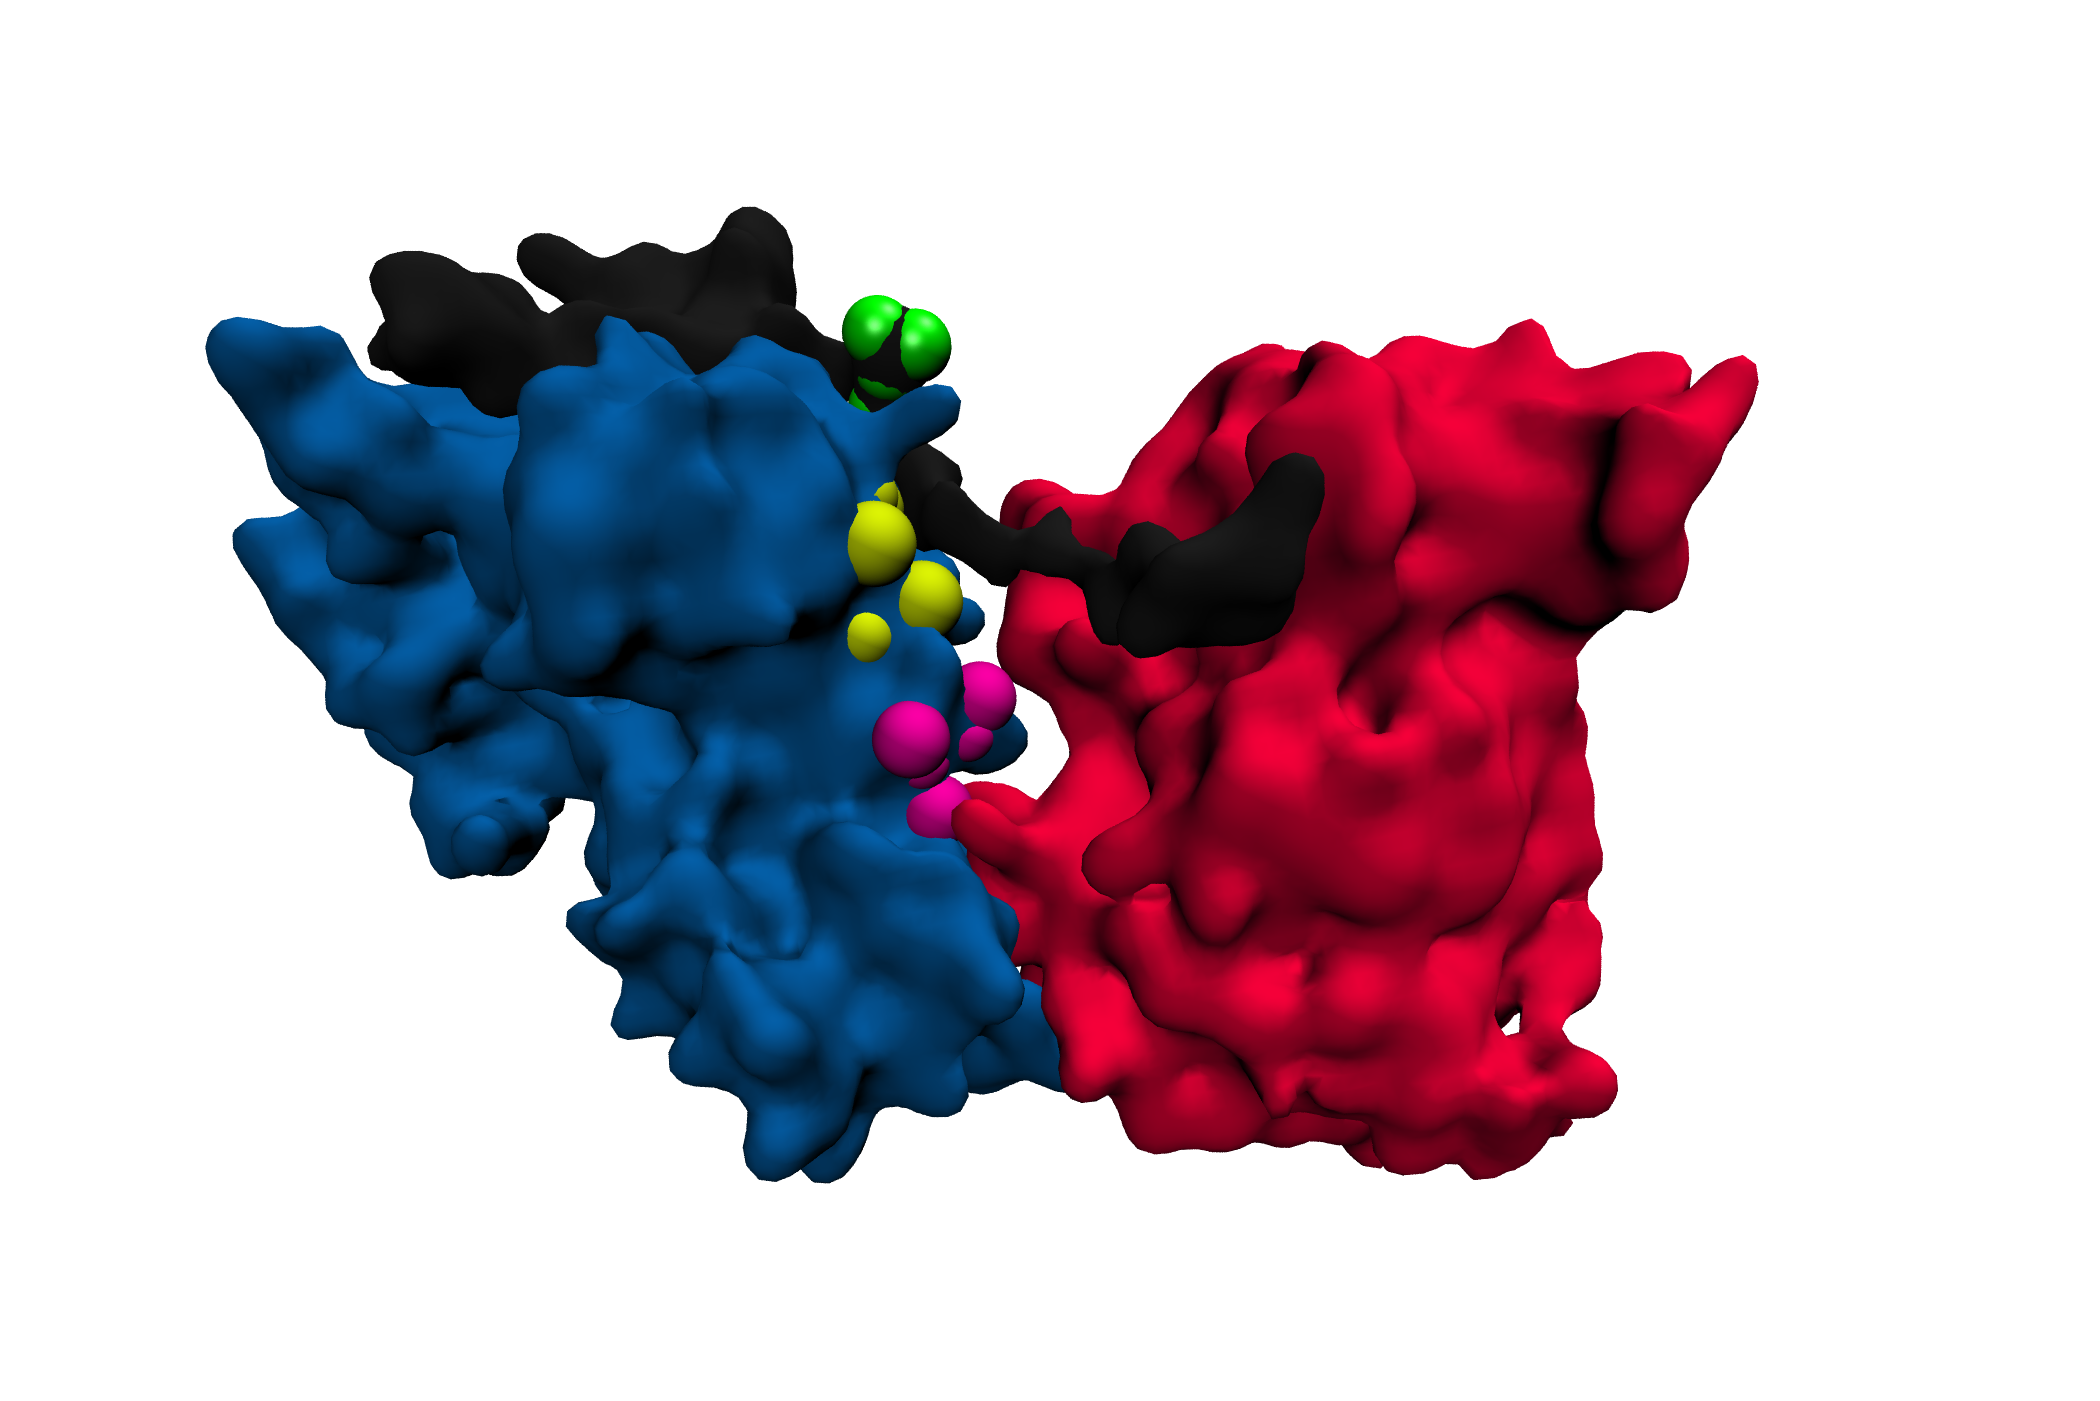
\includegraphics[height=4cm]{figures/results/fak_mem}
	\nicecaption{3D structure of FAK-MEM}{The 3D structure shows the FERM domain (blue), the kinase (red) and the linker (black, transparent). The membrane is not shown. The autophosphorylation site \acid{Y}{397} (green) is exposed. Residues around \acid{S}{47} (magenta) get farther away from the kinase, while residues around \acid{W}{52} (yellow) get closer.}
	\label{mem:3d}
\end{figure}
%
%
%
